% Diese Zeile bitte -nicht- aendern.
\documentclass[course=erap]{aspdoc}
\usepackage{amsmath}
\usepackage{algpseudocode}
\usepackage{algorithm}
%%%%%%%%%%%%%%%%%%%%%%%%%%%%%%%%%
%% TODO: Ersetzen Sie in den folgenden Zeilen die entsprechenden -Texte-
%% mit den richtigen Werten.
\newcommand{\theGroup}{102} % Beispiel: 42
\newcommand{\theNumber}{A301} % Beispiel: A123
\author{Balkis Nouri \and Yesmine Maalej \and Ismail Ben Ayed}
\date{Wintersemester 2020/21} % Beispiel: Wintersemester 2019/20
%%%%%%%%%%%%%%%%%%%%%%%%%%%%%%%%%
% Diese Zeile bitte -nicht- aendern.
\title{Gruppe \theGroup{} -- Abgabe zu Aufgabe \theNumber}

\begin{document}

\maketitle

\section{Einleitung}
In diesem Projekt geht es darum, die Wurzelfunktion in einer guter Nährung zu berechnen.
Der Näherungswert der Quadratwurzel wird verwendet, um zu ermitteln, wie viele
Personen es geben muss, damit mit einer Wahrscheinlichkeit von 0,5 mindestens zwei Personen
das gleiche Element aus einer Menge M von n Elementen teilen.
\\ Die Anzahl der Personen k lässt sich wie folgendes berechnen:
\begin{equation} \label{eq1}
    k \geq \frac{1+\sqrt{8n \cdot \ln{2}}}{2}
\end{equation}
wir beschäftigen uns im Rahmen unseres projekt mit der Berechnung von k für ein gegebenes n.
\\ Dafür implementieren wir bestimmte Verfahren um  die Wurzel $\sqrt{8n. \ln{2}}$ möglichst gut zu nähren.
Als reine Reihedarstellung, werden wir die Taylor Reihe implementieren. Danach werden wir eine Lookup methode entwickeln.
Schließlich, vergleichen wir die beide Verfahren mit dem Heron Verfahren,das auch implementiert wird.  \\
Im folgenden werden wir jedes Verfahren explizit darstellen und auf ihre Genauigkeit und  Performanz eingehen.
\section{Lösungsansatz}
Wir werden keine Näherung für den Logarithmus einsetzen weil wir floats verwerden. Die Wurzelfunktion hat ein float parameter
und deshalb die Näherung von der Logarithmus verloren wird. Aus diesem Grund werden wir ln(2) als $0.693147$ verwenden.
\subsection{Taylor Reihe:}
Als reine Reihe Darstellung bietet sich die Taylor Reihe, die für die Berechnung der Wurzel verwendet wird \cite{TaylorseriesApprox}:
\begin{equation} \label{eq2}
    f(x) = \sum_{n=0}^{\infty} \frac{f^{(n)}(a)(x-a)^n}{n!}  \approx {\sqrt{x}}
\end{equation}
Als konstante a wählen wir die Zahl 1 und damit ist die neue Gleichung die Folgende:
\begin{equation} \label{eq3}
    f(x) = \sum_{n=0}^{\infty} \frac{f^{(n)}(1)(x-1)^n}{n!}  \approx {\sqrt{x}}
\end{equation}
Weil die vorberechnete Reihe nur dann konvergiert wenn -1<x<1 ist \cite{TaylorExpansion}, müssen wir unser x entsprechend anpassen damit die Reihe anwendbar wird . Da unserer x der Wert $1+8n.\ln{2}$ entpricht ,müssen wir zuerst 1 von x substrahieren und dann x-1 zu einem wert zwischen -1 und 1 umwandeln . Unsere idee war, x zu y umzuwandeln wobei  $  y= x \cdot 10^{-l}$ und l = anzahl der ziffern in Zahl x .Damit ist x kleiner gleich 1.
\\Jetzt stellt sich die Frage wie kann man  die Taylor Reihe implementieren. Zuerst wollen wir die Koeffizienten herausfinden und
dann mit der Potenz von (x-1) multiplizieren.
\\ sei $a_{0}$ .. $a_{n}$ Koeffizienten von entsprechenden Termen. Dann ist
\\
$
    a_0=\frac{f^{(0)}(1)}{0!}
    =\frac{1^{\frac{1}{2}}}{0!}
    =1 ,
    a_1=\frac{f^{(1)}(1)}{1!}
    =\frac{1^{\frac{-1}{2}}\cdot \frac{1}{2} }{1!}
    =\frac{1}{2} ,
    a_2=\frac{f^{(2)}(1)}{2!}
    =\frac{1^{\frac{-3}{2}}\cdot \frac{1}{2} \cdot \frac{-1}{2} }{2!}
    =\frac{-1}{8}
$
wir zeigen nun per induktion dass

\begin{equation} \label{eq4}
    a_n=\frac{(-1)^{n-1} \cdot \prod_{i=1}^{(n-1)} (2i-1)}{2^{n} \cdot n!}
\end{equation}
gilt für alle n>=1.
\\ Induktionsbasis:Wir zeigen, dass die Formel für n=1 richtig ist:
\begin{center}
    $ a_1=\frac{f^{(1)}(1)}{1!} =\frac{1^{\frac{-1}{2}}\cdot \frac{1}{2} }{1!} =\frac{1}{2} $,  $\frac{(-1)^{0} \cdot \prod_{i=1}^0 1}{2^{1} \cdot 1!} =\frac{1}{2}$
\end{center}
Damit die Gleichung für n=1 gilt.\\
Induktionsschritt: wir nehmen an, dass die Behauptung für n gilt.Wir zeigen, dass die Formel auch für n+1 gilt:
\\ wir benutzen zuerst die Gleichung\footnote{Beweis siehe Beweis.pdf}:
\begin{equation} \label{eq5}
    f^{n+1}(x)=\frac{(\frac{1}{2}-n)\cdot  f^{n}(x)}{x}   mit f(x) =\sqrt{x}
\end{equation}
Dann ist :
\begin{center}\label{eq6}


    $
        a_{n+1}=\frac{f^{(n+1)}(1)}{(n+1)!}
        =\frac{(\frac{1}{2}-n)\cdot  f^{n}(1)  }{(n+1)!\cdot 1}
        =\frac{(\frac{1}{2}-n)\cdot  f^{n}(1)  }{n!\cdot (n+1)}
        = a_n \cdot \frac{(\frac{1}{2}-n)} {n+1}
    $
    \\
    $
        \stackrel{\text{IH}}{=}\frac{(-1)^{n-1}
            \cdot \prod_{i=0}^{(n-1)} (2i-1)}{2^{n} \cdot n!} \cdot \frac{\frac{1}{2}-n} {n+1}$
    \\
    $=\frac{(-1)^{n-1} \cdot \prod_{i=1}^{(n-1)} (2i-1)}{2^{n} \cdot n!} \cdot \frac{-(2n-1)}{2 \cdot (n+1)}$
    \\
    $=\frac{(-1)^{n} \cdot \prod_{i=1}^{(n)} (2i-1)}{2^{n+1} \cdot (n+1)!}$
\end{center}
Nun ist die Gleichung schon bewiesen. Aus dieser Formel können wir die folgende Gleichung ableiten:
\begin{equation}\label{eq7}
    a_{n}=(-1)^{n-1}\cdot \frac{\mid a_{n-1}\mid \cdot (2(n-1)-1)} {2 \cdot n}
\end{equation}
für n>=1.
\\ wir multiplizieren mit dem absoluten Wert von $a_{n}$, da das Vorzeichen zwischen negativ und positiv interpolieret, wenn der Index gerade bzw. ungerade ist.
\\ Da das Ergebnis eines Koeffizienten  vom vorherigen Koeffizienten abhängt, ist
die Verwendung von Simd  nicht möglich .Um SIMD zu vernwenden, müssen die Koeffizienten unabhängig berechenbar sein, was nicht der Fall in unserer Implementierung ist.
\\ Nun sind wir mit der Berechnung von $\sqrt{x\cdot 10^{-l}}$ fertig und wollen unser x
zu richtigem Format bringen, dafür müssen wir einige Rechenoperationen zuerst führen:
\begin{equation}\label{eq8}
    \sqrt{x\cdot 10^{-l}}  = \sqrt{x} \cdot \sqrt{10^{-l}}
    \Longrightarrow \sqrt{x}=\sqrt{x\cdot 10^{-l}}\cdot \sqrt{10^{l}}
\end{equation}
Um die Berechnung von $\sqrt{10^{l}}$ ohne die Verwendung von sqrt zu führen müssen wir zwei Fällen betrachten \cite{smallx}:
\\
1.Fall: l ist Gerade dann $\Longrightarrow \sqrt{10^{l}}$=$10^{l/2}$
\\
2: Fall: l ist ungerade dann $\Longrightarrow \sqrt{10^{l}}$=$10^{(l-1)/2} \cdot \sqrt{10}$
\\ Nun sind wir mit der Berechnung von $\sqrt{1+8nln(2)}$ fertig.
\subsection{Look-Up-Tabelle}
Die Technik besteht darin ~\cite{lut}, die höchstwertigen Bits der Mantisse
als Index für eine Wurzeltabelle zu verwenden. Durch Verwendung dieses nachgeschlagenen Wertes und
Halbierung des Exponenten kann eine Wurzelfunktion mit geringer Genauigkeit erstellt werden, die viel schneller läuft als die andere Methoden.
Wir werden nur die 15 höchstwertigen Bits der Mantisse in einem Array von shorts speichern damit es nicht viele Speicher benutzt.
Zur Veranschaulichung werden wir einen Fließkomazahl mit einem Acht-Bit-Exponenten(e), einem Ein-Bit-Vorzeichen und einer 15-Bit-Mantisse(m),gespeichert in der Form $2^{e_7..e_0} * 1.m_{14}..m_0$ betrachten.
\begin{equation} \label{eq9}
    \sqrt{2^{e}\cdot{m}}=2^{\frac{e}{2}}\cdot{\sqrt{m}}
\end{equation}
Gleichung (8) zeigt, dass die Wurzel von einer
Fließkommazahl darauf reduziert, den Exponenten zu halbieren und die Wurzel von der Mantisse zu ziehen.
Da ein ungerader Exponent nicht durch 2 geteilt werden kann,zerlegen wir die Zahl in einen geraden Exponenten $e_7..e_10$, und eine Mantisse $e_0m_{13}..m_0$ im Bereich [1..4).Dies speichert alle Werte von [1..4) ohne Informationsverluste
der ursprünglichen Fließkommadarstellung.
Deshalb werden wir eine Look-Up-Tabelle erstellen,die die Wurzeln der Werte $2^{e_0} \times 1.m_{14}..m_0$ speichert. Also sie besteht aus 2 Teilen, die Hälfte für sqrt(X) und die Hälfte für sqrt(2X). Im folgenden betrachten wir
den Algorithmus für die erstellung der Look-Up-Tabelle:
\begin{algorithm}[hbt!]
    \caption{build table()}\label{alg:cap1}
    \begin{algorithmic}
        \State $\textbf{for}  i: \textbf{integer}  0,2^{16}-1$
        \State $f \gets 1.i$
        \State $table[i] \gets mantissa(\sqrt{f});$
        \State $f \gets 2\cdot1.i$
        \State $table[i+2^{15}] \gets mantissa(\sqrt{f});$

    \end{algorithmic}
\end{algorithm}

Nach der Erstellung der Look Up Tabelle, werden wir die Gleichung (8) nutzen um die Wurzel zu finden.Im folgenden betrachten wir
den Algorithmus der Lookup Wurzel:


\begin{algorithm}[hbt!]
    \caption{LUT sqrt}\label{alg:cap2}
    \begin{algorithmic}
        \State $e \gets \textbf{exponent(V)}$
        \State $i \gets \textbf{mantissa(V)}$
        \If{(e \textbf{bit-and} 1)}  \Comment{der Exponent ist ungerade}
        \State das hohe Bit von i setzen
        \EndIf
        \State $e \gets \frac{e}{2}$  \Comment{Dividiere e durch zwei
            (Bei dieser Division muss das Vorzeichen erhalten bleiben)}
        \State $j \gets T[i] $
        \State  $U \gets 2^e \cdot 1.j  $


    \end{algorithmic}
\end{algorithm}
\subsection{Heron Verfahren}

Der Grundgedanke der Heron-Methode besteht darin, dass sie von einer ungefähren Schätzung ausgeht und ein neues ungefähres Ergebnis liefert, das besser ist als das erste. Dieser Vorgang kann so oft wiederholt werden, bis die gewünschte Genauigkeit erreicht ist.
Angenommen, wir wollen die Quadratwurzel aus n und nehmen eine erste Schätzung a vor, dann liegt $\sqrt{n}$ immer zwischen a und $\frac{n}{a}$ ~\cite{HeronLoesungsansatz}, da : \\
wenn a $\leq$ $\sqrt{n}$, dann ist $\frac{n}{a}$ $\geq$  $\sqrt{n}$ und
wenn  a $\geq$ $\sqrt{n}$, dann ist $\frac{n}{a}$ $\leq$  $\sqrt{n}$\\
O.B.d.A. betrachten wir den Fall  a $\leq$ $\sqrt{n}$: \\
a und n sind zwei positive Zahlen und  a $\leq \sqrt{n} \Longrightarrow
    \frac{1}{a} \geq \frac{1}{\sqrt{n}} \Longrightarrow \frac{n}{a} \geq \frac{n}{\sqrt{n}} \Longrightarrow \frac{n}{a} \geq \sqrt{n}$.\\
Betrachten wir vorerst einen beliebigen Anfangswert $a_{0}$. Folgend berechnen wir die Zahl $\frac{n}{a_0}$. Wie wir oben gezeigt haben, muss $\sqrt{n}$ irgendwo zwischen $a_0$ und $\frac{n}{a_0}$ liegen. Eine angemessenere Schätzung für $\sqrt{n}$ ist daher die Zahl, die genau zwischen $a_0$ und $\frac{n}{a_0}$ liegt, d.h das aritmetische Mittel:
\begin{equation}\label{eq10}
    a_1 = \frac{a_0 + \frac{n}{a_0}}{2}
\end{equation}
Diese Zahl setzen wir als neuen Wert $a_1$. Wir berechnen zunächst $a_2$,$a_3$,... in genau dieser Art und erhalten mit jedem Schritt eine besseren Näherung.\\
Eine weitere Sache, die zu beweisen ist, ist: als $i\rightarrow\infty , a_i\rightarrow\sqrt{n} $. Dazu müssen wir beweisen, dass~\cite{Heronsconvergence}:
\begin{equation}\label{eq11}
    \forall i\geq1 : a_i\geq\sqrt{n}
\end{equation}
Wir haben also:
$a_{i+1} = \frac{a_i + \frac{n}{a_i}}{2} \Leftrightarrow
    2a_{i}a_{i+1} = a_i^2 + n \Leftrightarrow
    a_i^2 - 2a_{i}a_{i+1}+a = 0$.
Dies ist eine quadratische Gleichung in $a_i$. Wir wissen, dass diese Gleichung eine reelle Lösung in Bezug auf $a_i$ haben muss, da $a_i$ explizit durch den iterativen Prozess konstruiert wurde.
Ihre Diskriminante ist also $b^2-4ac\geq0$, wobei: $a=1$ , $b=-2a_{i+1}$ , $c=n$. Das führt zu:
$ 4a_{i+1}^2-4n\geq0 \Rightarrow 4*(a_{i+1}^2-n)\geq0 \Rightarrow
    a_{i+1}^2 \geq n$. Da $a_0$ unsere anfängliche Vermutung für das Ergebnis der Quadratwurzel ist, wird es positiv sein, also ist $a_i \geq 0 ,\forall i_{\geq 0} $($a_i$ ist einfach das aritmetische Mittel zweier positiver Zahlen). Daher:
$  \forall i\geq0 : a_{i+1}\geq\sqrt{n} \Rightarrow
    \forall i\geq1 : a_i \geq \sqrt{n}$. Als nächstes betrachten wir:
$a_i-a_{i+1}=a_i - \frac{a_i + \frac{n}{a_i}}{2}=
    \frac{1}{2a_i}*(a_i^2-n)$. Hier kann man leicht erkennen, dass
$a_i-a_{i+1} \geq0$ for $i\geq1$. Daraus und aus Lemma (10) und unter der Voraussetzung, dass wir den ersten Term $a_0$ ignorieren (über den wir nichts aussagen können), ist die Folge $\langle a_i \rangle$ abnehmend und unten durch a begrenzt.
Dann konvergiert die Heron-Methode gegen $\sqrt{n}$.\\

Da die Wahl des Anfangsschatzes für die Performanz dieses Algorithmus wichtig ist, die wir später in Abschnitt 4 <Performanzanalyse> erörtern werden,
haben wir einige Berechnungen durchgeführt, um einen geeigneten Anfangsschatz zu erhalten. \\
Die Idee~\cite{initialguess} ist, eine erste Schätzung aus den Kandidaten $\{2, 7, 20, 70, 200, 700, ...\}$ auszuwählen, basierend auf der Tatsache, dass eine Quadratwurzel nur etwa halb so viele ganze Ziffern hat wie die Zahl selbst. Weiter erklärt, beginnt ein guter Schätzwert mit einer 2 oder einer 7 und hat etwa halb so viele Ziffern wie der ganzzahlige Teil von n, da: Eine Zahl mit k Ziffern liegt im Bereich $[10^{k-1}, 10^{k}[$. D.h. wenn eine Zahl 4 Ziffern hat, ist sie mindestens 1000 und weniger als 10000. Das arithmetische Mittel dieser Extremwerte beträgt $5*10^{k-1}$ und $\sqrt{5*10^{k-1}}$ = $\sqrt{5} * 10^{\frac{k}{2}} * 10^{-\frac{1}{2}}$. Hier betrachten wir zwei Fälle: \\
\begin{enumerate}
    \item  Wenn k gerade ist, erhält man $10^{k/2}$ mal 0.7071..., was nahe an $10^{k/2}*0.7$ liegt. Unsere Vermutung ist also eine Zahl, die mit 7 beginnt und k/2 Ziffern hat. D.h: $0.7*10^{k/2}$. \\
    \item  Wenn k ungerade ist, erhält man $\sqrt{5} * 10^{(k-1)/2}*10^{1/2}*10^{-1/2} = 10^{(k-1)/2}*2.236...$, was nahe an
          $10^{(k-1)/2}*2 = 10^{(k+1)/2}*0.2$ liegt. Unsere Vermutung ist also eine Zahl, die mit 2 beginnt und (k+1)/2 Ziffern hat. D.h: $0.2*10^{(k+1)/2}$. \\
\end{enumerate}
Da das arithmetische Mittel nicht alle Zahlen repräsentiert, was bedeutet, dass es Zahlen mit geraden Ziffern gibt, deren Quadratwurzel viel näher an einer Potenz von 10 mal 2 als an einer Potenz von 10 mal 7 liegt, haben wir beschlossen, der absolute Unterschied zwischen n (der Zahl, deren Quadratwurzel
berechnet werden soll ) und $2*10^{i}$ zu berechnen und sie dann mit den absoluten Unterschied von n und
$7*10^{i}$ zu vergleichen. Basierend auf dem kleinsten Unterschied, wählen wir unsere erste Schätzung aus.\\
Schließlich können wir diese Quadratwurzelannäherung nun in der Birthday-Paradox-Formel (1) anwenden.
\subsection{ Berechnung der glibc Wurzelfunktion}
Die Berechnung von glibc Wurzelfunktion beschreibt sich als eine Bit-für-Bit-Methode mit ganzzahliger Arithmetik.~\cite{glibc}
Im folgenden werden wir diese Methode in 3 Schritte beschreiben.
\begin{enumerate}
    \item Normalisierung :
          Skaliere x zu y in [1,4) mit geraden Potenzen von 2:
          Suche eine ganze Zahl k, so dass $1 <= (y=x*2^{2k}) < 4$, dann
          $sqrt(x) = 2^k * sqrt(y)$


    \item Bit-für-Bit-Berechnungen:
          Es sei $q_{i}=sqrt(y)$, abgeschnitten auf i Bit nach dem Binärpunkt ($q_{i} = 1$),
          \begin{equation} \label{eq12}
              s_{i}=2\times q_{i}, und \hspace{1mm} y_{i}=2^{i+1} \times (y-q_{i}^{2}).
          \end{equation}
          Um $q_{i+1}$ aus $q_{i}$ zu berechnen, prüft man, ob
          \begin{equation} \label{eq13}
              (q_{i}+2^{-(1+i)})^{2}<=y.
          \end{equation}
          Wenn (2) falsch ist, dann ist $q_{i+1}$ = $q_{i}$; sonst ist $q_{i+1} = q_{i} + 2$
          Mit etwas algebraischer Manipulation ist es nicht schwer zu sehen dass (2) äquivalent ist zu
          \begin{equation} \label{eq14}
              s_{i}+2^{-(1+i)}<=y_{i}.
          \end{equation}
          Der Vorteil von (3) ist, dass $s_{i}$ und $y_{i}$ wie folgt berechnet werden können
          mit der folgende Rekursionsformel:
          wenn (3) falsch ist
          \begin{equation} \label{eq15}
              s_{i+1}=s_{i} ,  y_{i+1}=y_{i}
          \end{equation}
          ansonsten,
          \begin{equation} \label{eq16}
              s_{i+1}=s_{i}+2^{-i} ,  y_{i+1}=y_{i}-s_{i}-2^{-(i+1)}
          \end{equation}
    \item Abschließende Rundung:
          Nachdem wir das Ergebnis von 24 Bits erhalten haben, berechnen wir noch ein Bit.
          Zusammen mit dem Rest können wir entscheiden, ob das
          Ergebnis genau ist, größer als 1/2ulp oder kleiner als 1/2ulp
          (es wird nie gleich 1/2ulp sein).
          Der Rundungsmodus lässt sich feststellen, indem man prüft, ob
          huge + tiny gleich huge ist, und ob huge - tiny gleich
          gleich huge ist für einige Fließkommazahlen huge und tiny.

\end{enumerate}
\subsection{Weitere Anwendungen der brithday eq formel:}
Die birthday-eq-Formel beschränkt sich nicht auf die Berechnung der Anzahl k von Personen,
so dass mindestens zwei Personen mit mindestens 0,5 Wahrscheinlichkeit den gleichen Geburtstag haben, sondern
geht sie auch  auf die Berechnung der Anzahl k von Personen, so dass mindestens zwei Personen mit mindestens 0,5
Wahrscheinlichkeit das gleiche Element aus einer Menge M mit n Elementen haben.In folgenden werden wir einige Beispiele zitieren
\subsubsection{Gleiche PIN}
Theoretisch gibt es $10000$ mögliche vierstellige Kombinationen von PIN,
in denen die Zahlen 0 bis 9 angeordnet werden können. Es bräuchte jedoch nur eine Gruppe von 119 Personen,
um die Wahrscheinlichkeit zu erhöhen, dass mindestens zwei Personen die gleiche PIN haben.
\subsubsection{Kollisionen bei MD5-Hashes}
Das Gleiche gilt für die Berechnung der Anzahl der MD5-Hashes. Der MD5 bildet $2^{128}$ verschiedene Werte ab.
Deshalb beträgt die Anzahl , damit zwei Hashes zufällig zusammenstoßen,etwa: $2.17\times 10^{19}$.
\subsection{ k in Abhängigkeit von n}
Nach der Berechnung von k für ein gegebenes n wäre es interessant zu untersuchen, wie die Beziehung zwischen k und n graphisch dargestellt werden kann. In der ersten Grafik würden wir k für n berechnen, wenn n<1000 ist. Beim Testen schien ein 200er Intervall die Daten besser darzustellen.
Im zweiten Diagramm betrachten wir größere Werte, beginnend mit  $10^5$ und mit einem Intervall von $3*10^5$ zwischen den Werten.\\
Aus den Graphen lässt sich schließen, dass mit zunehmender Anzahl der Elemente n der Menge auch die Anzahl der Personen steigt, die mit einer Wahrscheinlichkeit von 0,5 die gleichen Elemente haben.
\begin{figure}[h!]
    \centering
    \begin{minipage}{.5\textwidth}
        \centering
        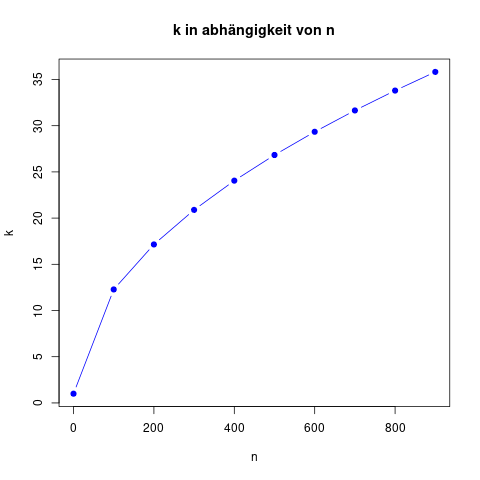
\includegraphics[width=.9\linewidth]{graphs/firstgraph.png}

        \label{fig:test1}
    \end{minipage}%
    \begin{minipage}{.5\textwidth}
        \centering
        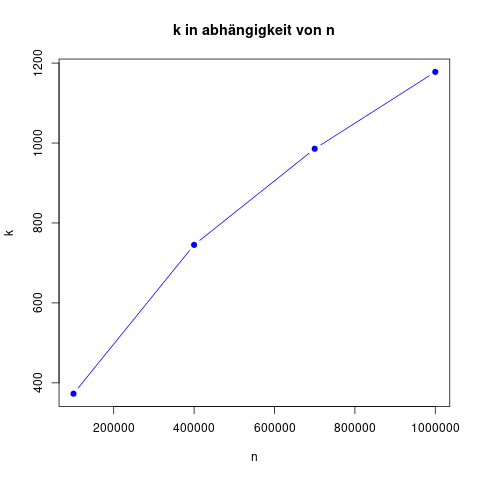
\includegraphics[width=.9\linewidth]{graphs/sndgraph.png}

        \label{fig:test2}
    \end{minipage}
\end{figure}
% TODO: Je nach Aufgabenstellung einen der Begriffe wählen
\section{Genauigkeit}
\subsection{Genauigkeit der Taylor Reihe}
Der $n^\text{th}$  Grades des Taylor-Polynoms bei x=a ist \cite{errortaylor}:
\begin{equation} \label{eq17}
    P_{n}(x)=f(a)+\frac{f^{1}(a)}{1!}(x-a)+...+\frac{f^{n}(a)\cdot (x-a)^{n}}{n!}
\end{equation}
Da die Taylor-Approximation umso genauer wird, je mehr Terme enthalten sind, ist $P_{n+1}(x)$
genauer :
\begin{equation} \label{eq18}
    P_{n+1}(x)=f(a)+\frac{f^{1}(a)}{1!}(x-a)+...+\frac{f^{n}(a)\cdot(x-a)^{n}}{n!}+\frac{f^{n+1}(a)\cdot (x-a)^{n+1}}{(n+1)!}
\end{equation}
\begin{equation}
    =P_{n}(x)+\frac{f^{n+1}(a)\cdot (x-a)^{n+1}}{(n+1)!}
\end{equation}
Da die Differenz zwischen $P_{n+1}$ und $P_{n}$ nur der letzte Term ist, kann der Fehler nicht größer sein als dieser Term . Mit anderen Worten  der Fehler $R_{n}$ ist:
\begin{equation} \label{eq19}
    R_{n}=max(\frac{f^{n+1}(a)}{(n+1)!} \cdot (x-a)^{n+1})
\end{equation}
Weil n und a konstanten sind ,bleiben die Terme, die nur von diesen Konstanten und x abhängen,vom max Operator unberührt und können nach außen gezogen werden :
\begin{equation} \label{eq20}
    R_{n}=\frac{max(f^{n+1}(a))}{(n+1)!} \cdot (x-a)^{n+1}
\end{equation}
Der größte Wert, der mit $f^{n+1}$ eruzeugt wird kann den maximalen Wert dieser Ableitung nicht überschreiten.
Nennen Sie den x-Wert, der diesen Maximalwert liefert, z, und der Fehler wird:
\begin{equation} \label{eq21}
    R_n(x)=\frac{f^{(n+1)}(z)}{(n+1)!}(x-a)^{n+1}.
\end{equation}

\subsection{Genauigkeit der Look-Up-Tabelle}
Die Genauigkeit der Look-Up Wurzel hängt von der größe der Tabelle ab. Wir haben uns entschlossen, nur  die  15 Höchstwertigen bits
der Mantisse in einem Array von shorts zu speichern.Wir könnten auch alle bits von der Mantisse speichern um eine bessere Genauigkeit
zu erhalten.In diesem Fall müssen wir jedoch die type von die Tabelle ändern, da short nur maximal 16 bits enthalten kann.
Diese Erweiterung im Gegenteil benötigt mehr Speicher und deshalb ist sie ineffizient.
\subsection{Genauigkeit der Heron Verfahren}
Um die Genauigkeit der Heron-Methode zu analysieren, sollten wir zuerst die Fehlerquote bei einer Iteration mit der Fehlerquote bei der nächsten Iteration verknüpfen und sie vergleichen. Wir definieren also: $u_{i} = x_{i} - x$.
Dabei ist $x_{i}$ der Wert nach Iteration i und x ist das erwartete Ergebnis von $\sqrt{n}$, wobei n die Zahl ist, deren Wurzel wir suchen. Dann versucht man, $u_{i+1}$ in Abhängigkeit von $u_{i}$ zu setzen. Dafür verwenden wir die Gleichung (9) : $x_{i+1} = \frac{1}{2}*(x_{i}+\frac{n}{x_{i}})$ im Folgenden~\cite{HeronsGenauigkeit}:\\
$ u_{i+1} = x_{i+1} - x = \frac{1}{2}*(x_{i}+\frac{n}{x_{i}}) -  \frac{1}{2}*(x +\frac{n}{x})= \frac{1}{2}*(u_{i}+\frac{n}{x_{i}}-\frac{n}{x})=
    \frac{1}{2}*(u_{i}+\frac{n*(x-x_{i})}{x*x_{i}})$.\\
Da $x = \sqrt{n}$ dann $n = x^{2}$. Das führt uns zu:
$u_{i+1} = \frac{1}{2}*(u_{i}-\frac{x*u_{i}}{x_{i}}) = \frac{1}{2}*u_{i}*(1-\frac{x}{x_{i}}) \Rightarrow \\
    u_{i+1} = \frac{1}{2}*\frac{u_{i}^{2}}{x_{i}}$.
Berechnet man nun die Fehlerquote in Bezug auf x (=$\sqrt{n}$), die beträgt: \\
$e_{i} = \frac{u_{i}}{x} $. Daher: $e_{i+1} = \frac{u_{i+1}}{x} = \frac{1}{2}*\frac{u_{i}^{2}}{x*x_{i}} = \frac{1}{2}*\frac{u_{i}^{2}*x}{x^{2}*x_{i}} =
    \frac{1}{2}*e_{i}^{2}*\frac{x}{x_{i}} =
    \frac{1}{2}*e_{i}^{2}*\frac{1}{\frac{x_i}{x}} =
    \frac{1}{2}*e_{i}^{2}*\frac{1}{1-\frac{x}{x}+\frac{x_i}{x}}\Rightarrow e_{i+1} = \frac{1}{2}*e_{i}^{2}*\frac{1}{1+e_{i}}$.
Daraus kann man schließen, dass wenn $x_{i} \geq x $ dann $e_{i+1} \leq \frac{1}{2}*e_{i}$, da in diesem Fall : $e_{i+1} = |e_{i+1}| = \frac{1}{2}*e_{i}^{2}*\frac{1}{1+e_{i}}$ und $1+e_{i} \geq e_{i} \Rightarrow \\
    \frac{1}{1+e_{i}} \leq \frac{1}{e_{i}}
    \Rightarrow \frac{e_{i}}{1+e_{i}} \leq 1 \Rightarrow  \frac{e_{i}^{2}}{1+e_{i}} \leq e_{i} \Rightarrow e_{i+1}  \leq \frac{1}{2}*e_{i} $.  \\
Somit wird der relative Fehler bei jeder Iteration um einen Faktor kleiner als $\frac{1}{2}$ verringert, unabhängig davon, wie groß der anfängliche Fehler sein mag. Daraus lässt sich schließen, dass sich die Anzahl der richtigen Ziffern bei jedem Schritt im Wesentlichen verdoppelt, sobald $x_{i}$ größer als $\sqrt{n}$ wird.
Aus dem Lemma (10), das wir in Abschnitt 2.3 bewiesen haben: $ \forall i\geq1 , x_{i}\geq\sqrt{n}$.
Dazu nehmen wir ein Beispiel k= 2 in unserer Funktion birthdayeq, die $0.5+\sqrt{0.25+2*k*ln(2)}$ zurückgibt. In der nachstehenden Tabelle sind die richtigen Ziffern in jeder Iteration durch Fettdruck gekennzeichnet.
\begin{table}[h!]
    \centering
    \begin{tabular}{c|c}
        \textbf{$x_{i}$} & \textbf{apoximation of $\sqrt{0.25+2*k*ln(2)}$} \\
        \hline
        $x_0$            & 2.000000000000000000000                         \\
        $x_1$            & \textbf{1.7}55646944046020507812                \\
        $x_2$            & \textbf{1.738}642334938049316406                \\
        $x_3$            & \textbf{1.738559246063232421875}                \\
        $x_4$            & \textbf{1.738559246063232421875}                \\
    \end{tabular}
    \caption{die Entwicklung von $\sqrt{n}$ bei jeder Iteration}
    \label{tab:my_label}
\end{table} \\
Wie wir sehen können, ändert sich $x_i$ nach einer bestimmten Anzahl von Iterationen nicht mehr. Das liegt an der IEEE-754 Darstellung von \textit{float} und seiner begrenzten Genauigkeit. Wie wir wissen, verliert ein \textit{float} umso mehr an Präzision, je größer es ist. Wir haben also das kleinste Argument geprüft, das unsere Heron-Methode haben kann, nämlich $0.25+2*0*ln(2)=0.25$ und wir haben das kleinste \textit{float} berechnet, das man zu $\sqrt{0.25}=0.5$ addieren oder subtrahieren kann, damit es sich tatsächlich ändert. Diese Zahl ist 0.000000000000000000000000001(binär) = 0.000000059605(dezimal).
Und deshalb haben wir die Genauigkeit $x_i-x_{i+1}= 0.00000005$ gewählt.
\subsection{Vergleich der Genauigkeit}
\begin{table}[h!]
    \centering
    \begin{tabular}{|| c c c c ||}
        \hline
        n         & Heron             & Taylor                     & Lookup                     \\ [2ex]
        \hline\hline
        0         & 1.000000          & \textbf{1.000000}          & \textbf{1.000000}          \\
        1         & 1.779177          & \textbf{1.77917}9          & \textbf{1.77917}5          \\
        $10^5$    & 372.830017        & \textbf{372.83}2520        & \textbf{372.8}20312        \\
        $10^{10}$ & 117741.484375     & \textbf{11774}2.265625     & \textbf{1177}38.500000     \\
        $10^{15}$ & 37232968.000000   & \textbf{3723}3216.000000   & \textbf{37232}640.000000   \\
        ULongMax  & 3575794432.000000 & \textbf{3575}842560.000000 & \textbf{35757}75232.000000 \\
        [2ex]

        \hline
    \end{tabular}
\end{table}
Wie gezeigt bietet das Heron Verfahren die beste Genauigkeit an. Danach kommt die Taylor Reihe
und letzlich die LookUpTabelle ausser einige Ausnahmen.\\
Die Wahl dieses Beispiels beruht auf der Tatsache, dass je größer die Float-Zahl ist, desto mehr verliert sie beim Runden an Präzision. Dies ist auf die IEEE 745-Darstellung zurückzuführen. Deshalb haben wir Beispiele gewählt, die zu klein, klein, mittel, groß, zu groß sind.

\section{Performanzanalyse}
In unserem Projekt haben wir verschiedene Algorithmen und Ansätze benutzt. In diesem
Abschnitt werden wir einige Unterschiede zwischen diesen Algorithmen erläutern.
Getestet wurde auf einem System mit einem Intel(R) Core(TM) i7-10510U CPU, 1.80GHz GHz ,16 GB
Arbeitsspeicher, Ubuntu 20.04.3 LTS, 64 Bit, Linux-Kernel 5.11.0. Kompiliert wurde mit GCC
9.3.0 mit der Option-O3.
\subsection{LookUpTabelle}
Look-Up Tabelle ist ein praktisches Werkzeug zur Beschleunigung von Operationen,
die als Funktionen eines ganzzahligen Arguments ausgedrückt werden können. Sie verwenden gespeicherte,
vorberechnete Ergebnisse, die es dem Programm ermöglichen, sofort ein Ergebnis zu erhalten,
ohne die zeitaufwändige Operation erneut durchführen zu müssen.
Die ganze Prozess von unsere Lookup Tabelle kann, sobald die Tabelle erstellt ist, mit einem bitweisen Und,
zwei bitweisen Oder, einem bitweisen Test und fünf Verschiebeoperationen durchgeführt werden. Die Zeitkomplexität in diese Methode ist O(1).Deshalb unabhängig von n, bleibt immer die Zeitkomplexität dieselbe.
\subsection{TaylorReihe}
Die Implementierung der Taylor-Reihe enthält 3 Schleifen. Die erste Schleife bestimmt die Anzahl der Ziffern vor dem Dezimalkomma unseres x, was in $O(log(x))$ durchläuft. Im schlimmsten Fall beträgt die Zahl 20 Ziffern (Anzahl der Ziffern des ULONGMAX).
Die zweite Schleife hat i Durchlaüfe => O(i) und erreicht im schlimmsten Fall 50 .
Die letzte Schleife dauert höchstens O(Anzahl der Ziffern
+2)/2, was im schlimmsten Fall gleich 11 ist => O(11)
Insgesammt ist die Laufzeitkomplexität im Worst Case O(log(n)+i+log(n)) = O(log(n)+i)
\subsection{Heron Verfahren}
Die Heron-Methode ist eine bemerkenswert einfache und schnell konvergierende Methode zur Annäherung an die Quadratwurzel, da sie die Anzahl der richtigen Ziffern in jeder Iteration verdoppelt.
Wie in Abschnitt 2.3 erlautert wurde, liegt die Wahl unseres ersten Wertes $x_0$ nahe am Ergebnis $\sqrt{n}$. Daher brauchen wir nur ein paar Iterationen, um einen $x_i$ zu erhalten, dessen erste Ziffer mit dem Ergebnis $\sqrt{n}$ übereinstimmt.Außerdem haben wir vor der Schleife $x_0$ und $x_1$ bestimmt
und in Kenntnis von, dass unser Ergebnis $\sqrt{n}$ maximal 9 signifikante Ziffern hat, da die IEEE 745 Darstellung eines Floats uns mindestens 6 und höchstens 9 signifikante Ziffern liefert~\cite{HeronsPerformanz}, benötigen wir maximal $\lceil log_2(9)  \rceil +1$ Iterationen.(die letzte iteration ist zu bestimmen, dass das vorherige x korrekt ist). Damit verbleiben maximal 5 Iterationen, um zu unserem Ergebnis zu gelangen, sobald die erste korrekte Ziffer erscheint.\\
Außerdem hat unser Algorithmus eine Schleife, um die Anzahl der Ziffern vor dem Dezimalpunkt von n zu zählen, die maximal 20 sein kann, da ULONGMAX 20 Ziffern hat.
Wir können also sagen, dass die Zeitkomplexität dieser Schleife O(log(n)) ist. \\
Weitere Optimierungen mit SIMD sind aufgrund der Loop-carried Dependencies in unserem Algorithmus nicht möglich. \\
Zusammenfassend können wir sagen, dass unser Worst-Case-Szenario eine Zeitkomplexität von $O(\lceil log_2(Significantdigits(n))  \rceil) + O(log(n)) $ hat, was wir als optimierte Methode zur Annäherung an die Quadratwurzel betrachten können.
\subsection{Vergleich der verschiedenen Implementierungen}
\begin{figure}[H]
    \centering
    \begin{minipage}{.4\textwidth}
        \centering
        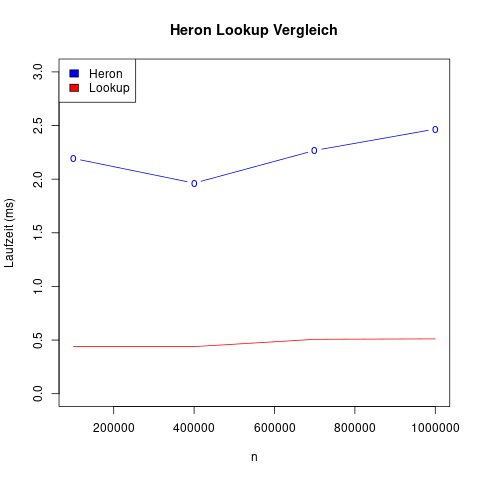
\includegraphics[width=.9\linewidth]{graphs/Heronlookup.png}
        \label{fig:test3}
    \end{minipage}%
    \begin{minipage}{.4\textwidth}
        \centering
        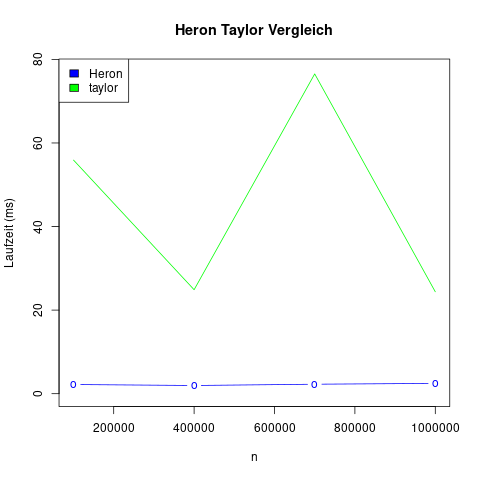
\includegraphics[width=.9\linewidth]{graphs/HeronTaylor.png}
        \label{fig:test4}
    \end{minipage}%
    \begin{minipage}{.4\textwidth}
        \centering
        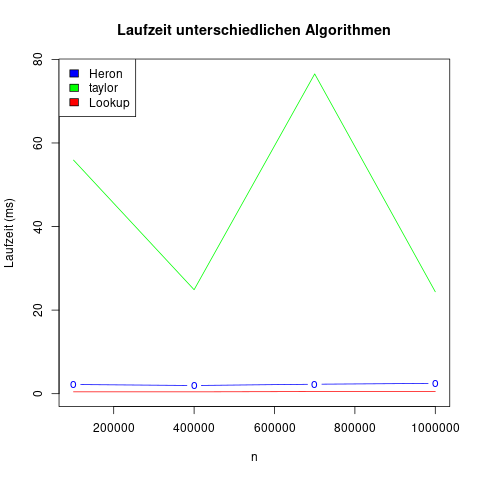
\includegraphics[width=.9\linewidth]{graphs/Allalgorithms.png}
        \label{fig:test5}
    \end{minipage}

\end{figure}
Nach Blick auf die Graphen fällt uns auf ,dass die LookUpTabelle die geringere Laufzeit anbietet. Danach kommt das Heron Verfahren
und letzlich die Taylor Reihe.

\section{Zusammenfassung und Ausblick}
In diesem Projekt haben wir die Wurzelfunktion durch verschiedene Rechenvorschriften
berechnet. Als Hauptimplementierung  verwenden wir das Heron Verfahren, da es die beste
Genauigkeit anbietet und eine mittlere Laufzeit hat. Als reine Reihedarstellung bietet sich die Taylor Reihe,
diese dauert länger als das Heron Verfahren und hat eine mittlere Genauigkeit.
Die Look up Tabelle ist im gegenteil das schnellste aber geringere Genauigkeit anzeigt.
Man kann auch andere effizienteren Algorithmen verwenden, wie das Goldschmidt's algorithm, um
die Laufzeit weiter zu beschleunigen. Man kann auch die Implementierung anpassen,
um inverse QuadratWurzel zu approximieren.

% TODO: Fuegen Sie Ihre Quellen der Datei Ausarbeitung.bib hinzu
% Referenzieren Sie diese dann mit \cite{}.
% Beispiel: CR2 ist ein Register der x86-Architektur~\cite{intel2017man}.

\bibliographystyle{plain}
\bibliography{Ausarbeitung}{}

\end{document}
